\section{Intermediate Representation (IR)} \label{sec:ir}

Compilers and programs that work with source code usually do not operate directly on the source code itself. They instead use \acrlong{ir}s (\acrshort{ir}) with different levels of abstraction. \cite[p.~1]{chow2013} Another benefit of using \acrshort{ir}s is that these are usually independent of code formatting, which allows the analysis and transformation only based on the syntax and semantics. Doing these on the actual code is error prune \cite{rustcdev2020.syntax}. This section summarizes the concept of two graph-based IR. The construction process of these representations is not documented as part of this paper.

\subsection{Abstract Syntax Tree (AST)} \label{sec:ir.ast}

An \acrfull{ast} is an abstract representation of the syntactic structure of source code in the form of a tree graph. Each node represents an item based on the formal definition of the language and the use case that the \acrshort{ast} is intended for. Edges between these nodes represent the hierarchical structure and logical connection of items. \cite[p.~22,~26]{slonneger1995} Figure \ref{fig:ast.simple-expr} is an example \acrshort{ast} visualization of the expression \texttt{3 * 3 + (5 - 2)}. The root of the tree is the \texttt{+} expression, as this is also the last one that will be evaluated. The \texttt{*} and \texttt{-} nodes are both sub nodes which intern have the integer literals as leaves.

\begin{figure}[H]
    \Tree[.\texttt{+} 
            [.\texttt{*} 3 3 ]
            [.\texttt{-} 5 2 ]]
    \caption[AST for a simple expression]{An example \acrshort{ast} for the expression: \texttt{3 * 3 + (5 - 2)}}
    \label{fig:ast.simple-expr}
\end{figure}

Branching expressions like loops and if statements have all branches as children, even if they are unreachable \cite[p.~28]{slonneger1995}. The existence inside the graph therefore does not imply that each expression will be executed. Figure \ref{fig:ast.if} illustrates an \acrshort{ast} for an \texttt{if} expression with two branches. However, most languages will only evaluate one branch based on the condition evaluation.

\begin{figure}[H]
    \begin{minipage}{0.5\textwidth}
        \centering
        \begin{verbatim}


            if true then
                return 0
            else
                return 5
            end
        \end{verbatim}
    \end{minipage}%
    \begin{minipage}{0.5\textwidth}
        \centering
        \Tree[.\texttt{if} 
                [.\texttt{true} ]
                [.\texttt{return} 0 ]
                [.\texttt{return} 5 ]]
    \end{minipage}
    \caption[AST for an if expression]{An example \texttt{if} expression with a corresponding \acrshort{ast}}
    \label{fig:ast.if}
\end{figure}

\newpage

\subsection{Control-Flow Graph (CFG)} \label{sec:ir.cfg}

The execution order of a program can be represented as a directed and connected graph called the \acrfull{cfg}. Compilers use these graphs for data flow analysis and performance optimization. The nodes of a \acrshort{cfg} represent basic building blocks of a program, like single statements. Edges connecting the nodes represent the possible execution paths that a program can take. \cite[p.~2]{allen1970} Figure \ref{fig:cfg.simple} shows an example program and the corresponding \acrshort{cfg}.

\begin{figure}[H]
    \centering
    \begin{minipage}{.5\textwidth}
        \centering
        \begin{verbatim}

            if false then
                print "hello"
            end

            print " "

            for x in 1..3 do
                print "world"
            end

            print "!"
        \end{verbatim}
    \end{minipage}%
    \begin{minipage}{.5\textwidth}
        \centering
        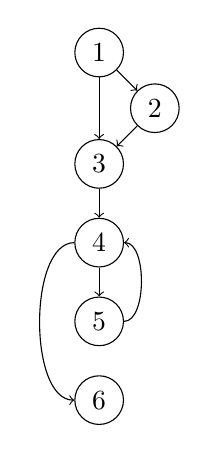
\begin{tikzpicture}[main/.style = {draw, circle}] 
            % if
            \node[main] (1) {1};
            \node[main] (2) [below right of=1] {2};
            \node[main] (3) [below left of=2] {3};
            \draw[->] (1) -- (2);
            \draw[->] (2) -- (3);
            \draw[->] (1) -- (3);
            
            % for
            \node[main] (4) [below of=3] {4};
            \node[main] (5) [below of=4] {5};
            \draw[->] (3) -- (4);
            \draw[->] (4) -- (5);
            \draw[->] (5) to [out=0,in=0,looseness=0.75] (4);
            
            % end
            \node[main] (6) [below of=5] {6};
            \draw[->] (4) to [out=180,in=180,looseness=0.75] (6);
        \end{tikzpicture}
    \end{minipage}
    \caption[CFG example]{An example program with a corresponding \acrshort{cfg}}
    \label{fig:cfg.simple}
\end{figure}

